\begin{frame}
\frametitle{Aufgabe 2}
\framesubtitle{Tiefpassfilter 1. Ordnung}
\begin{figure}[H]
\begin{center}
        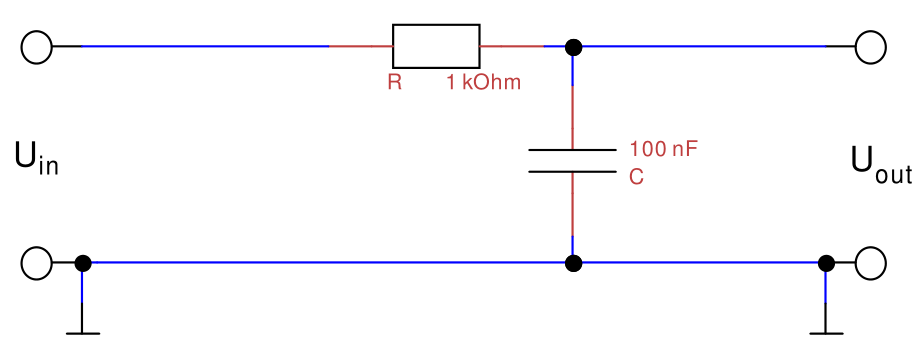
\includegraphics[scale=0.2]{./img/2a_bode_schaltbild.png}
\end{center}
\end{figure}
\end{frame}
\begin{frame}
    \frametitle{Tiefpassfilter 1. Ordnung}
    \framesubtitle{100Hz}
     \begin{figure}[H]
     \begin{center}
             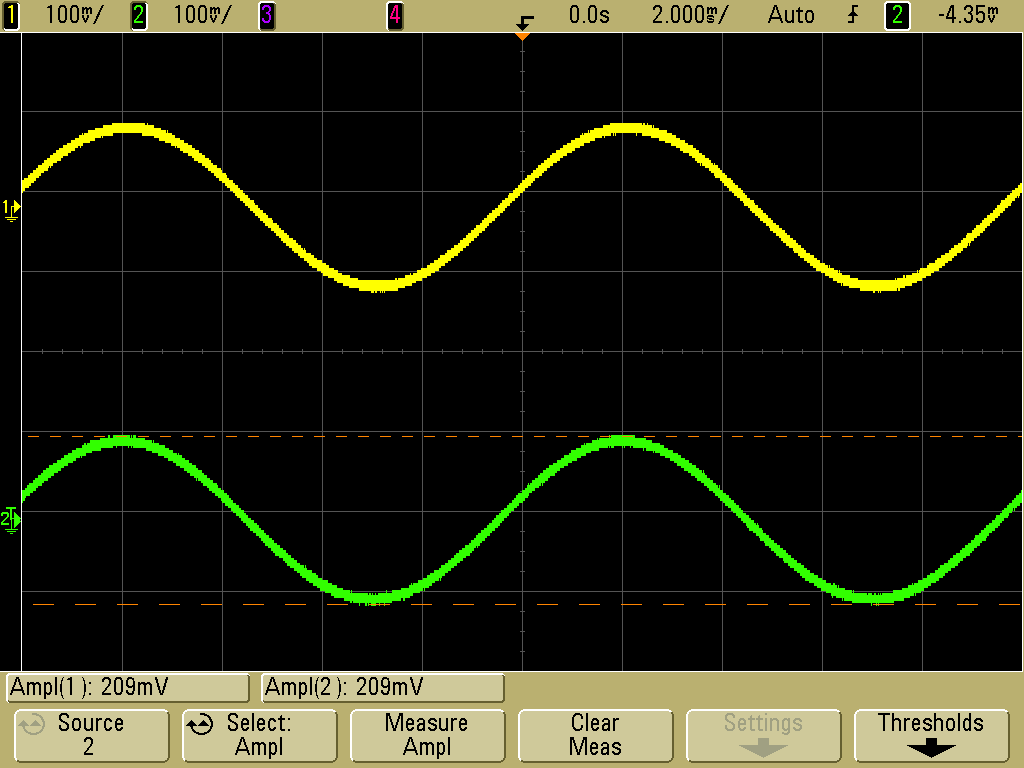
\includegraphics[scale=0.2]{./img/2a_Tief_100Hz.png}
     \end{center}
     \end{figure}
\end{frame}
\begin{frame}
    \frametitle{Tiefpassfilter 1. Ordnung}
    \framesubtitle{1.6kHz}
     \begin{figure}[H]
     \begin{center}
             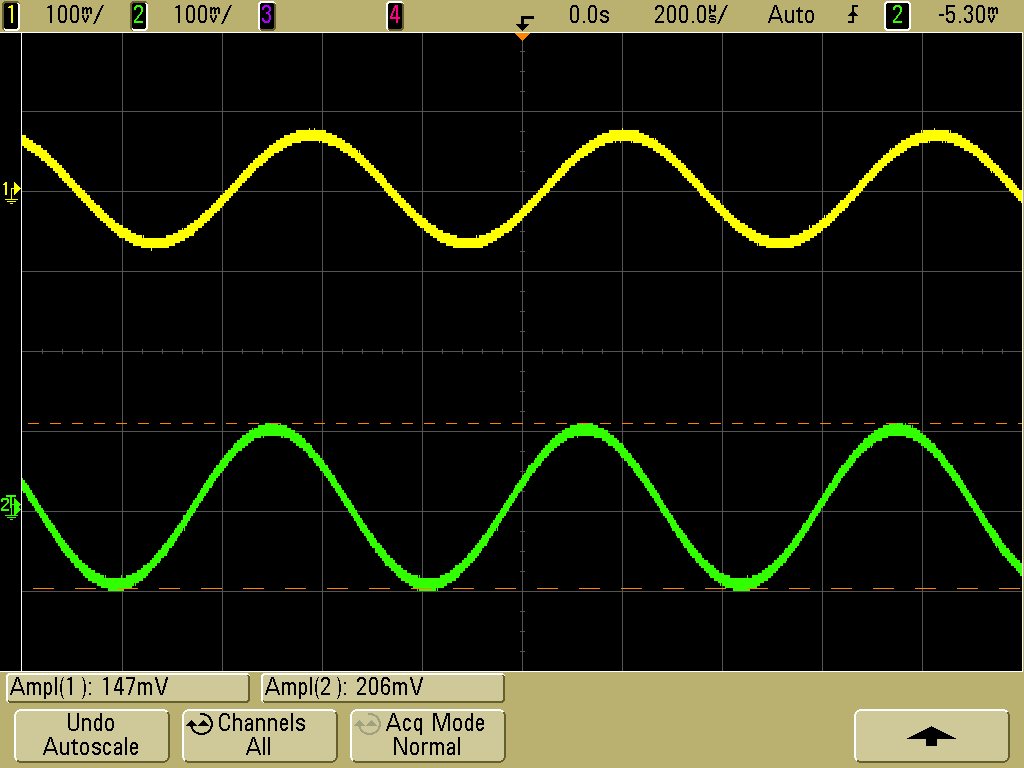
\includegraphics[scale=0.2]{./img/2a_Tief_1_6_kHz.png}
     \end{center}
     \end{figure}
\end{frame}
\begin{frame}
    \frametitle{Tiefpassfilter 1. Ordnung}
    \framesubtitle{1MHz}
     \begin{figure}[H]
     \begin{center}
             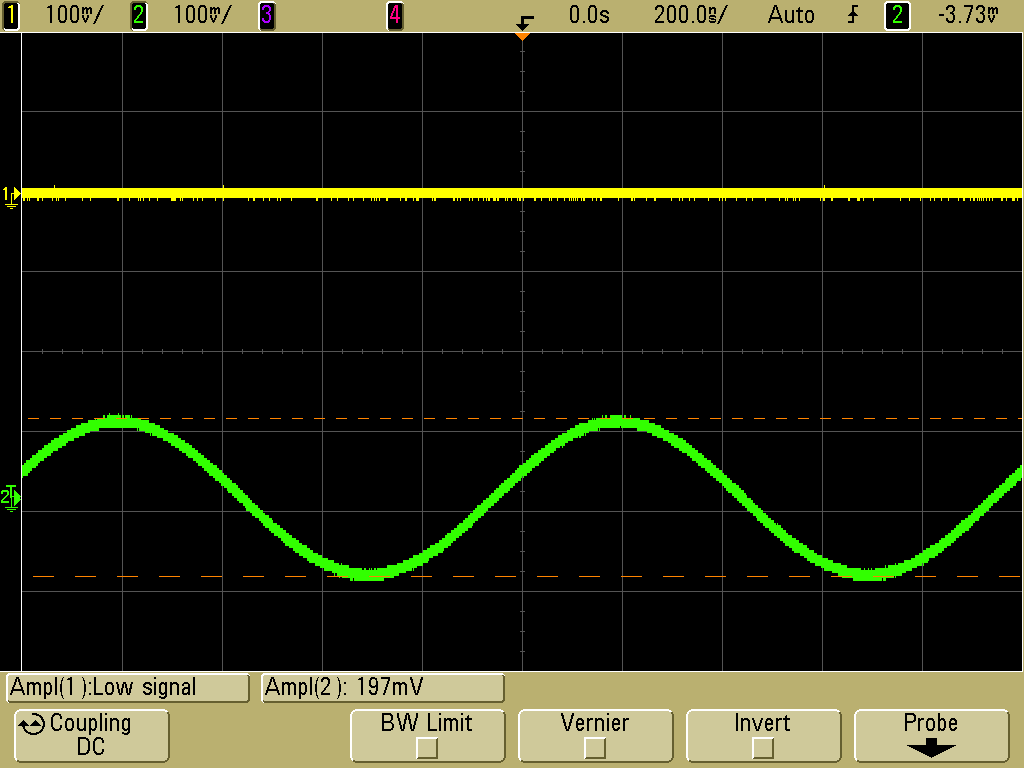
\includegraphics[scale=0.2]{./img/2a_tief_1MHz.png}
     \end{center}
     \end{figure}
\end{frame}
\begin{frame}
\frametitle{Aufgabe 2}
\framesubtitle{Bode Diagramm}
    \begin{itemize}
        \item Bode Diagramm: Auftragung Dämpfung über Frequenz
        \item Visualisierung von Dämpfung
        \item Dezibel:
    \end{itemize}
    \begin{equation*}
        V^* = 20 \log_{10} \left( \frac{U_2}{U_1} \right) 
    \end{equation*}
\end{frame}
\begin{frame}
\frametitle{Aufgabe 2}
\framesubtitle{Frequenzfilter}
    \begin{itemize}
        \item Hoch-,Tief-,Sperr-,Bandpassfilter
        \item Unterdrückung von Frequenzbereichen
        \item Ordnung gibt an wie stark die Dämpfung ausfällt: 1. Ordnung:
        $6db$ pro Oktave, 2. Ordnung $12dB$ pro Oktave etc.
        \item nichtlineares Verhalten
    \end{itemize}
\end{frame}
\begin{frame}
\frametitle{Aufgabe 2}
\framesubtitle{Tiefpass 1. Ordnung}
\begin{figure}[H]
\begin{center}
        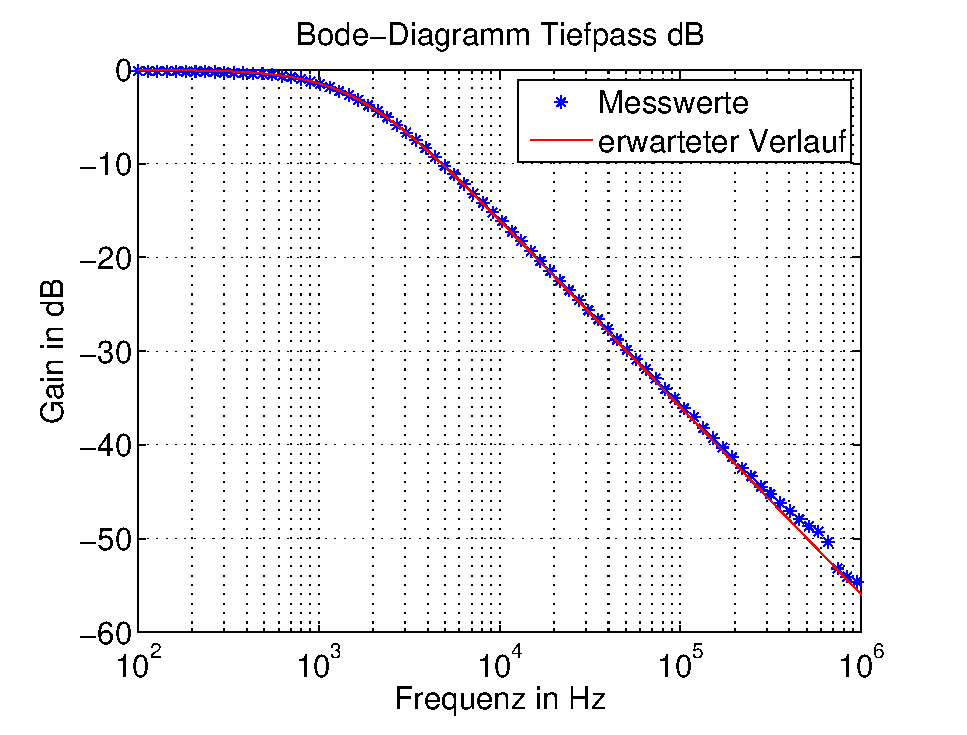
\includegraphics[scale=0.45]{./img/2a_bode_tief_dB.eps}
\end{center}
\end{figure}
\begin{itemize}
    \item Erwarteter Verlauf:
\end{itemize}
    \begin{equation*}
        V = 20 \log_{10} \left( \frac{1}{\sqrt{1+(\omega C R)^2}}\right)
    \end{equation*}
\end{frame}
\begin{frame}
\frametitle{Aufgabe 2}
\framesubtitle{Tiefpass 1. Ordnung}
\begin{figure}[H]
\begin{center}
        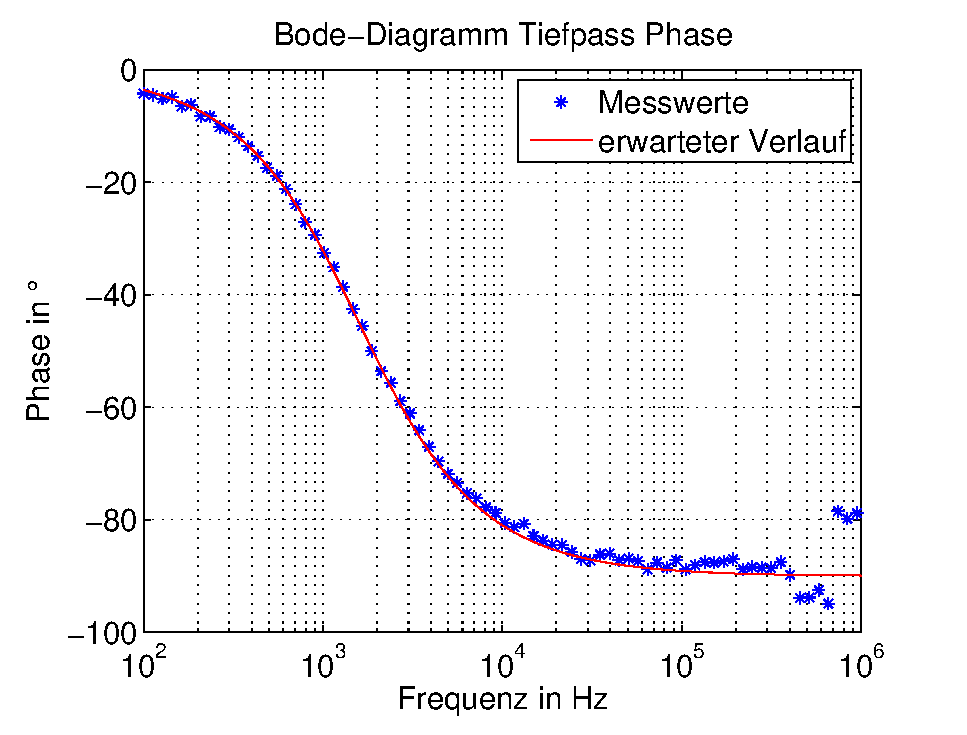
\includegraphics[scale=0.50]{./img/2a_bode_tief_phase.eps}
\end{center}
\end{figure}
\begin{itemize}
    \item Erwarteter Verlauf:
\end{itemize}
\begin{equation*}
    \varphi = - \arctan \left( \omega C R \right)
\end{equation*}
\end{frame}
\begin{frame}
    \frametitle{Aufgabe 2}
    \framesubtitle{Tiefpass 1. Ordnung}
\begin{itemize}
    \item $3dB$-Frequenz: linearer Abfall des Signals
    \item $\frac{U_{in}}{U_{out}}=\frac{1}{\sqrt{2}}$
    \item Theoretische Grenzfrequenz: $f_{c_T} = \frac{1}{2 \pi C R} \approx
    1591.55Hz$
    \item Aus Bode Diagramm bei $dB=3.185845$: $f_{c_T} \approx 1656 Hz$
\end{itemize}
\end{frame}
\begin{frame}
    \frametitle{Aufgabe 2}
    \framesubtitle{Tiefpass 1. Ordnung}
     \begin{itemize}
         \item Bestimmung der Steigung:
     \end{itemize}
     \begin{figure}[H]
     \begin{center}
             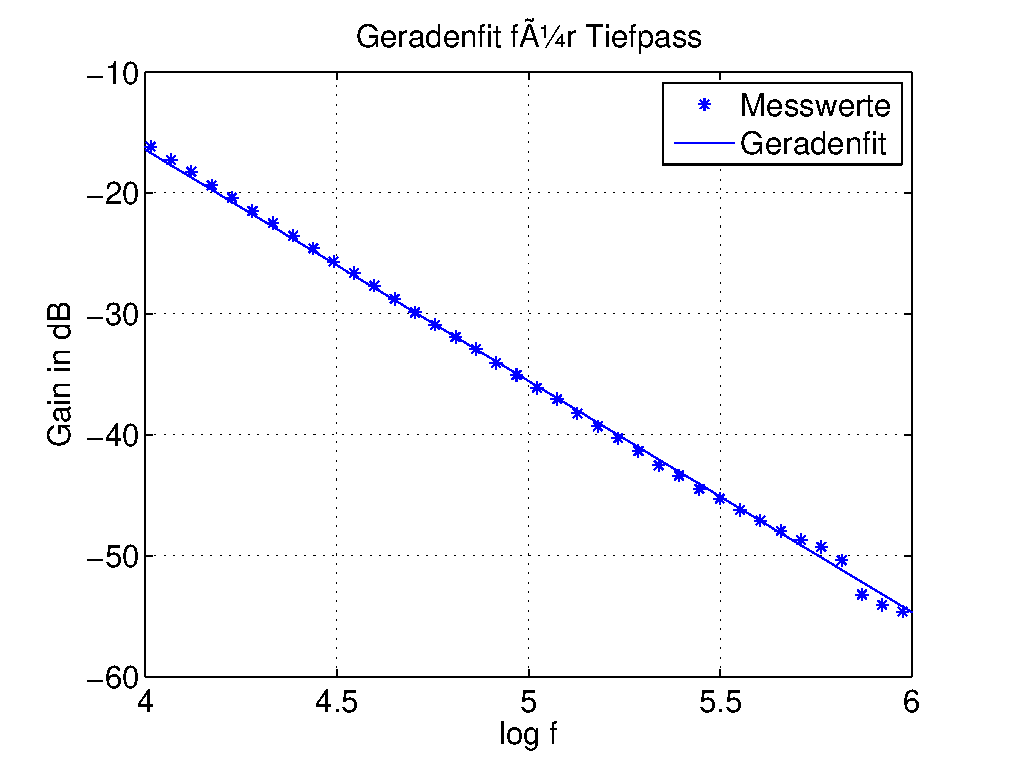
\includegraphics[scale=0.55]{./img/2a_Fit.eps}
     \end{center}
     \end{figure}
\end{frame}
\begin{frame}
    \frametitle{Aufgabe 2}
    \framesubtitle{Tiefpass 1. Ordnung}
     \begin{itemize}
        \item Fit Wert: $-19.12 \frac{dB}{Dekade}= -5.74 \frac{dB}{Oktave}$
        \item Theoretischer Wert:
        $-20\frac{dB}{\text{Dekade}}=-6\frac{dB}{\text{Oktave}}$
     \end{itemize}
\end{frame}
\begin{frame}
    \frametitle{Aufgabe 2}
    \framesubtitle{Hochpass 1. Ordnung}
     \begin{figure}[H]
     \begin{center}
             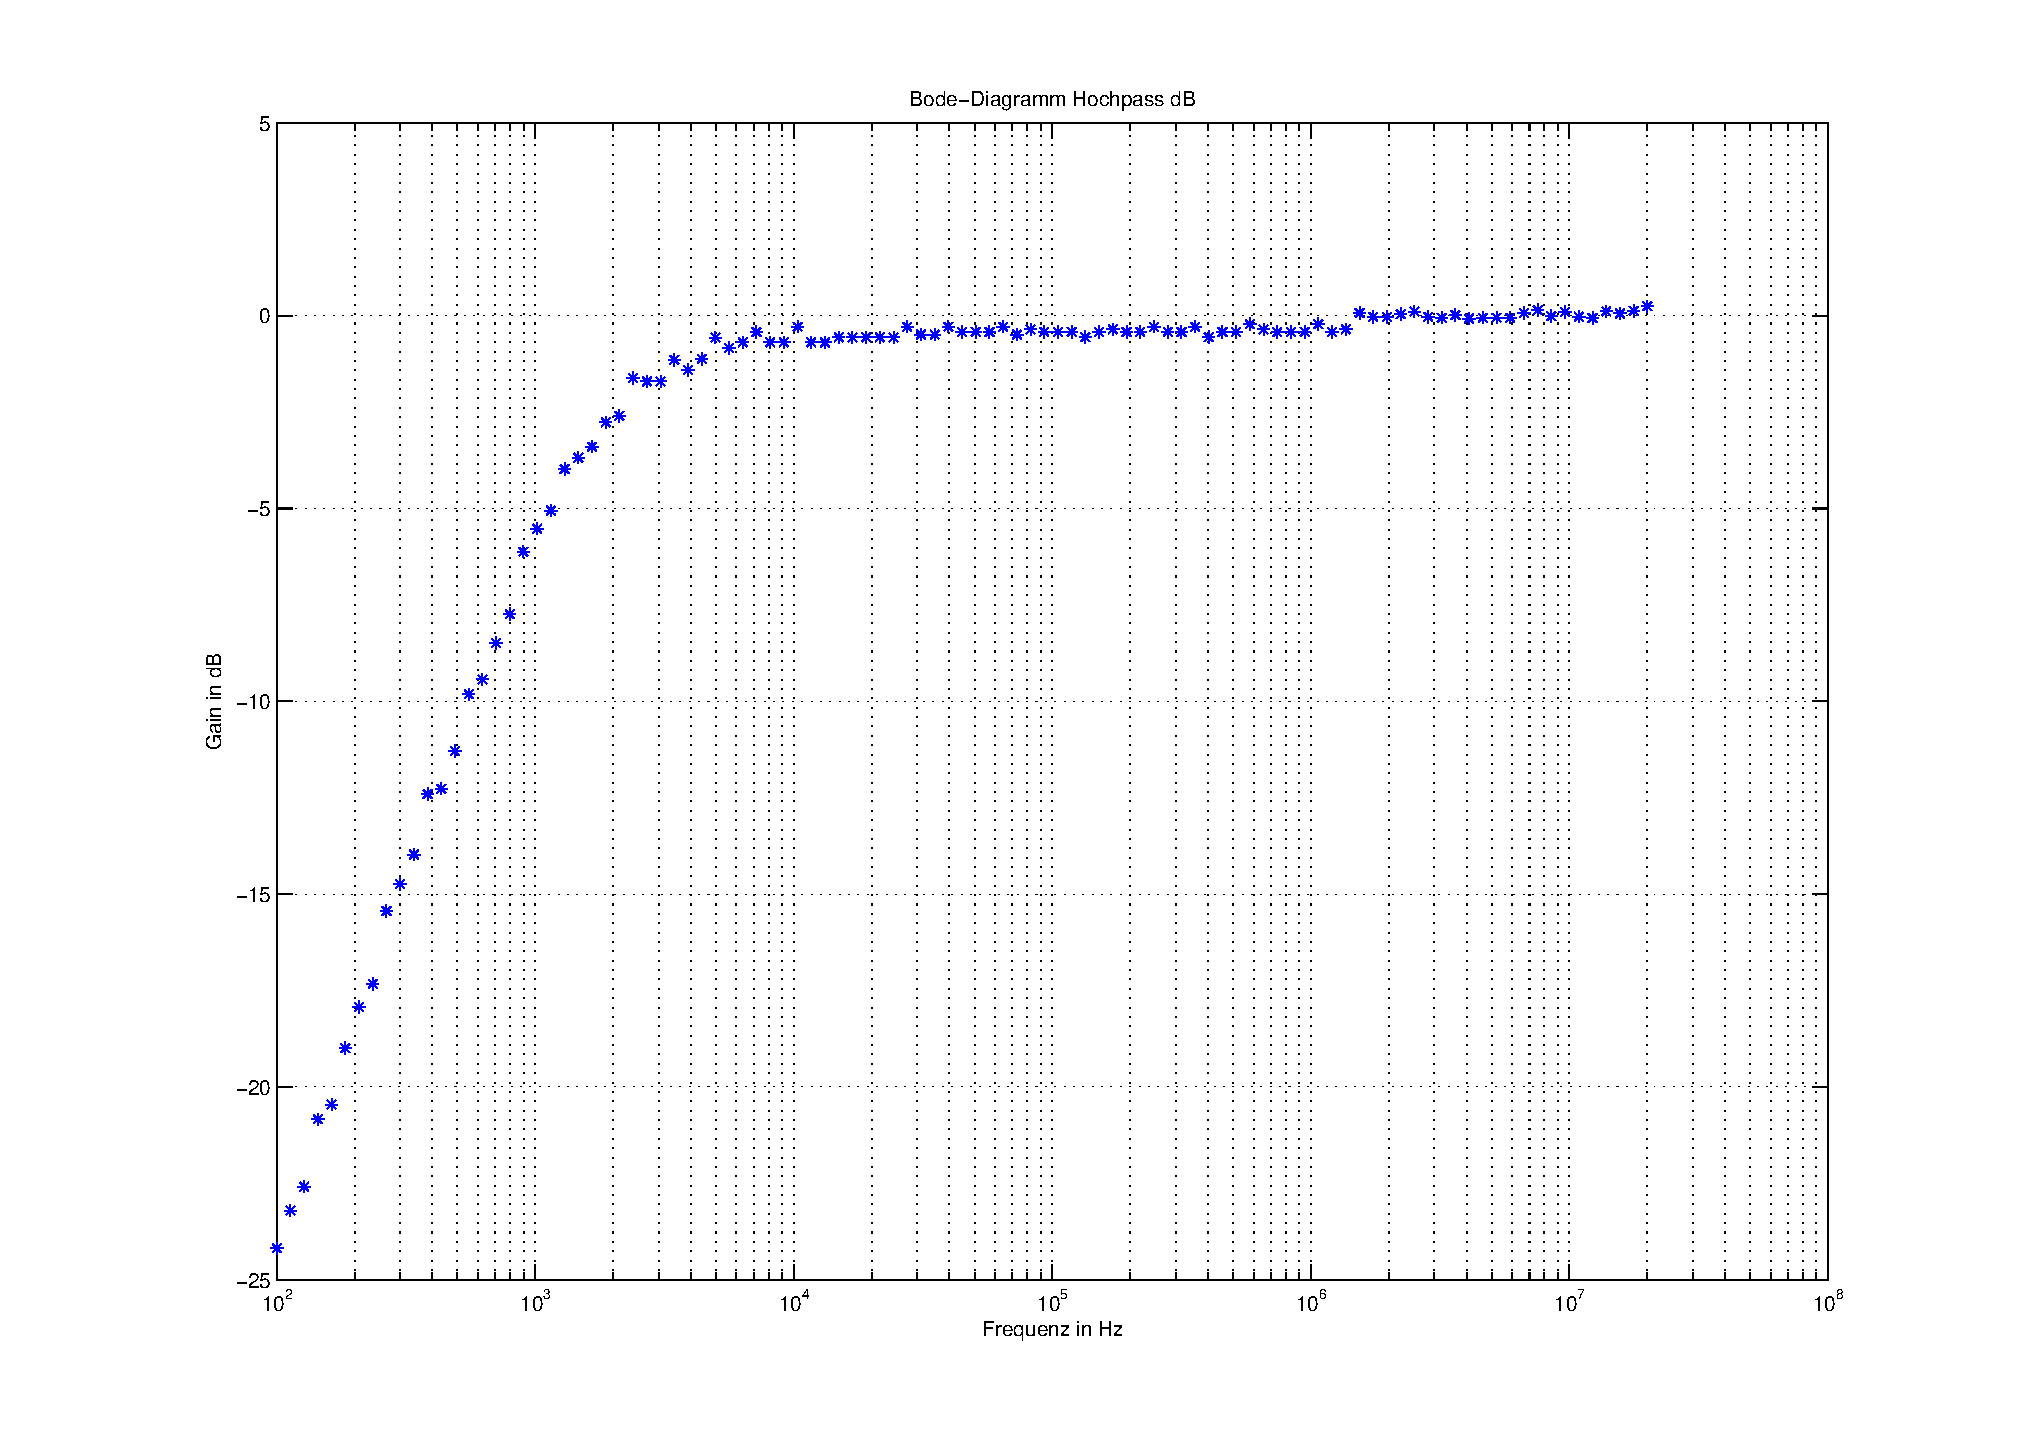
\includegraphics[scale=0.6]{./img/2b_bode_hoch_dB.eps}
     \end{center}
     \end{figure}
\end{frame}
\begin{frame}
    \frametitle{Aufgabe 2}
    \framesubtitle{Hochpass 1. Ordnung}
     \begin{figure}[H]
     \begin{center}
             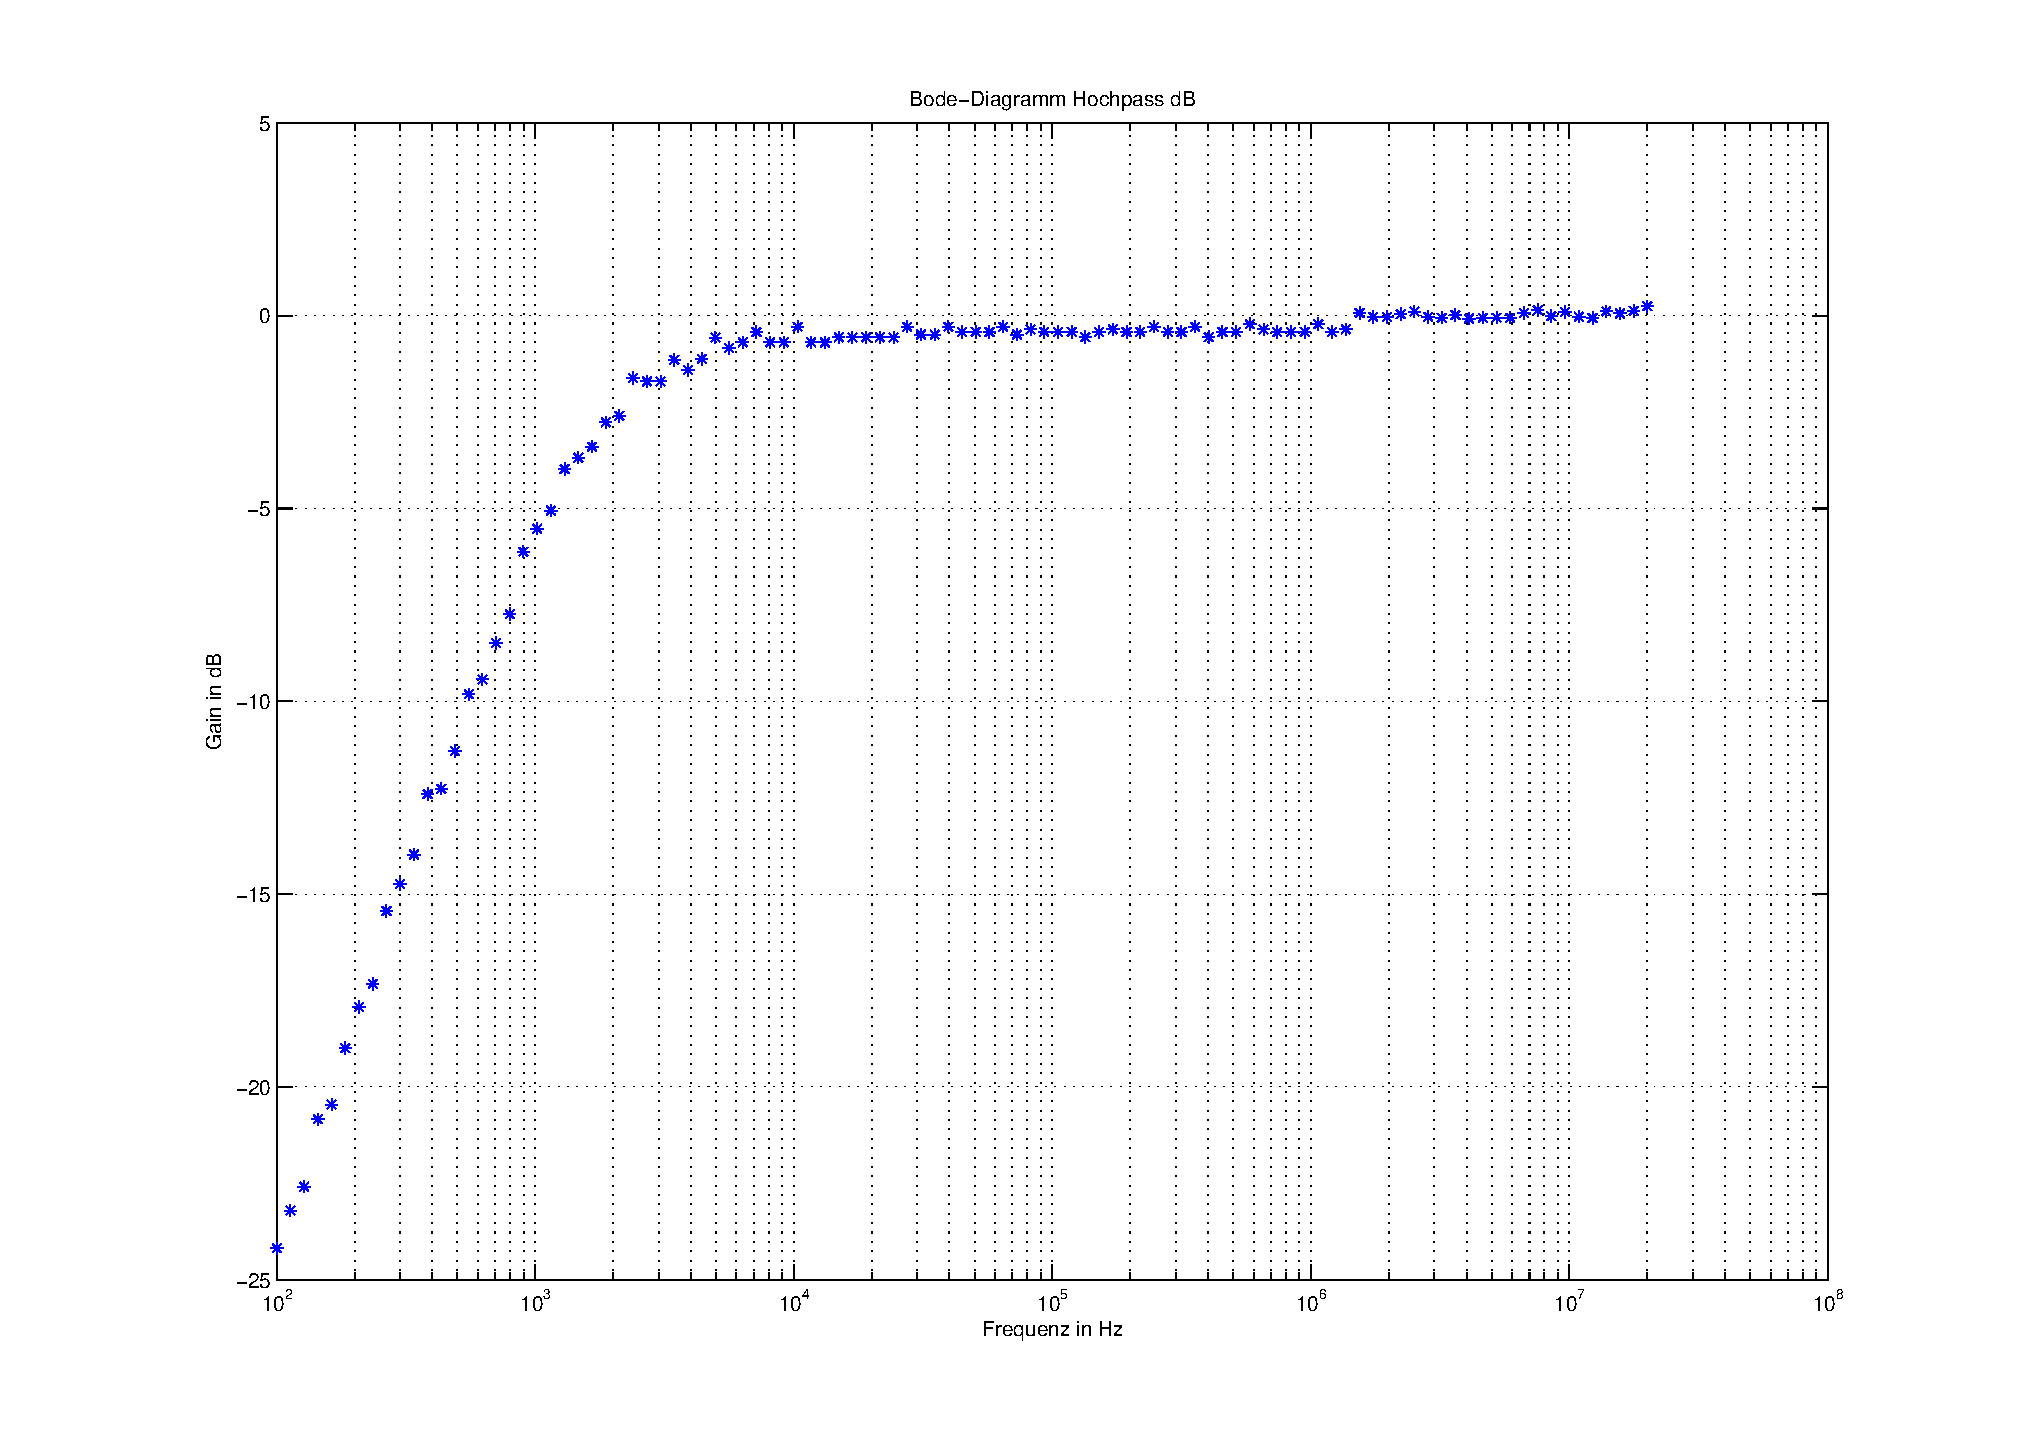
\includegraphics[scale=0.45]{./img/2b_bode_hoch_dB.eps}
     \end{center}
     \end{figure}
     \begin{itemize}
         \item Erwarteter Verlauf: 
     \end{itemize}
     \begin{equation*}
            V = 20 \log_{10} \left( \frac{\omega C R}{\sqrt{1 + (\omega C
            R)^2}}\right)
     \end{equation*}
\end{frame}
\begin{frame}
    \frametitle{Aufgabe 2}
    \framesubtitle{Hochpass 1. Ordnung}
     \begin{figure}[H]
     \begin{center}
             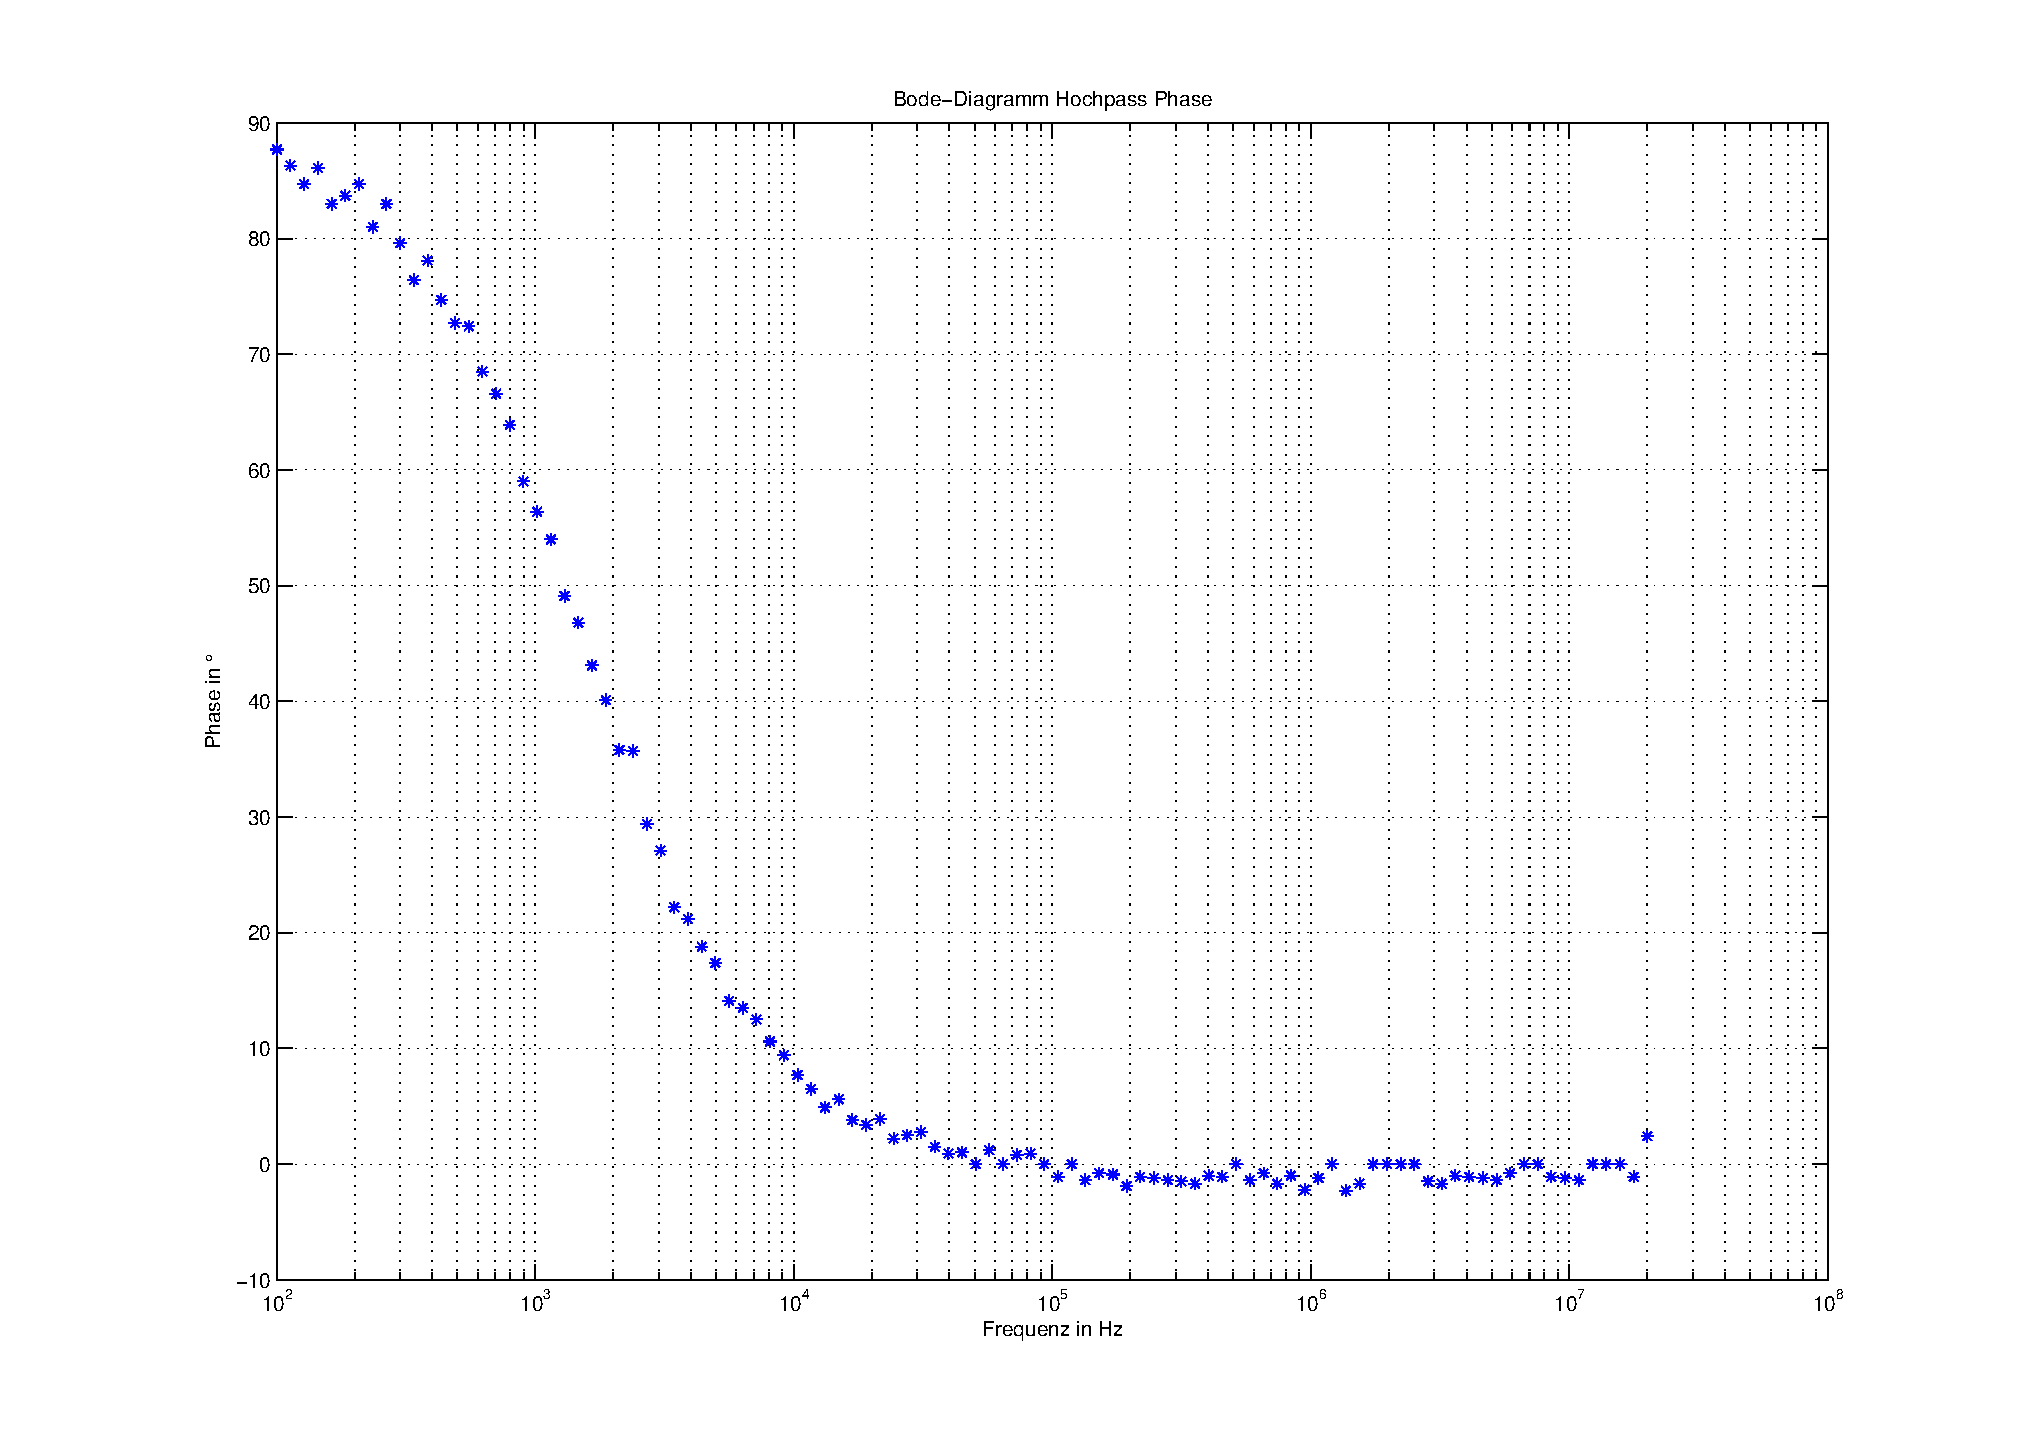
\includegraphics[scale=0.60]{./img/2b_bode_hoch_phase.eps}
     \end{center}
     \end{figure}
\end{frame}
\begin{frame}
    \frametitle{Aufgabe 2}
    \framesubtitle{Hochpass 1. Ordnung}
     \begin{figure}[H]
     \begin{center}
             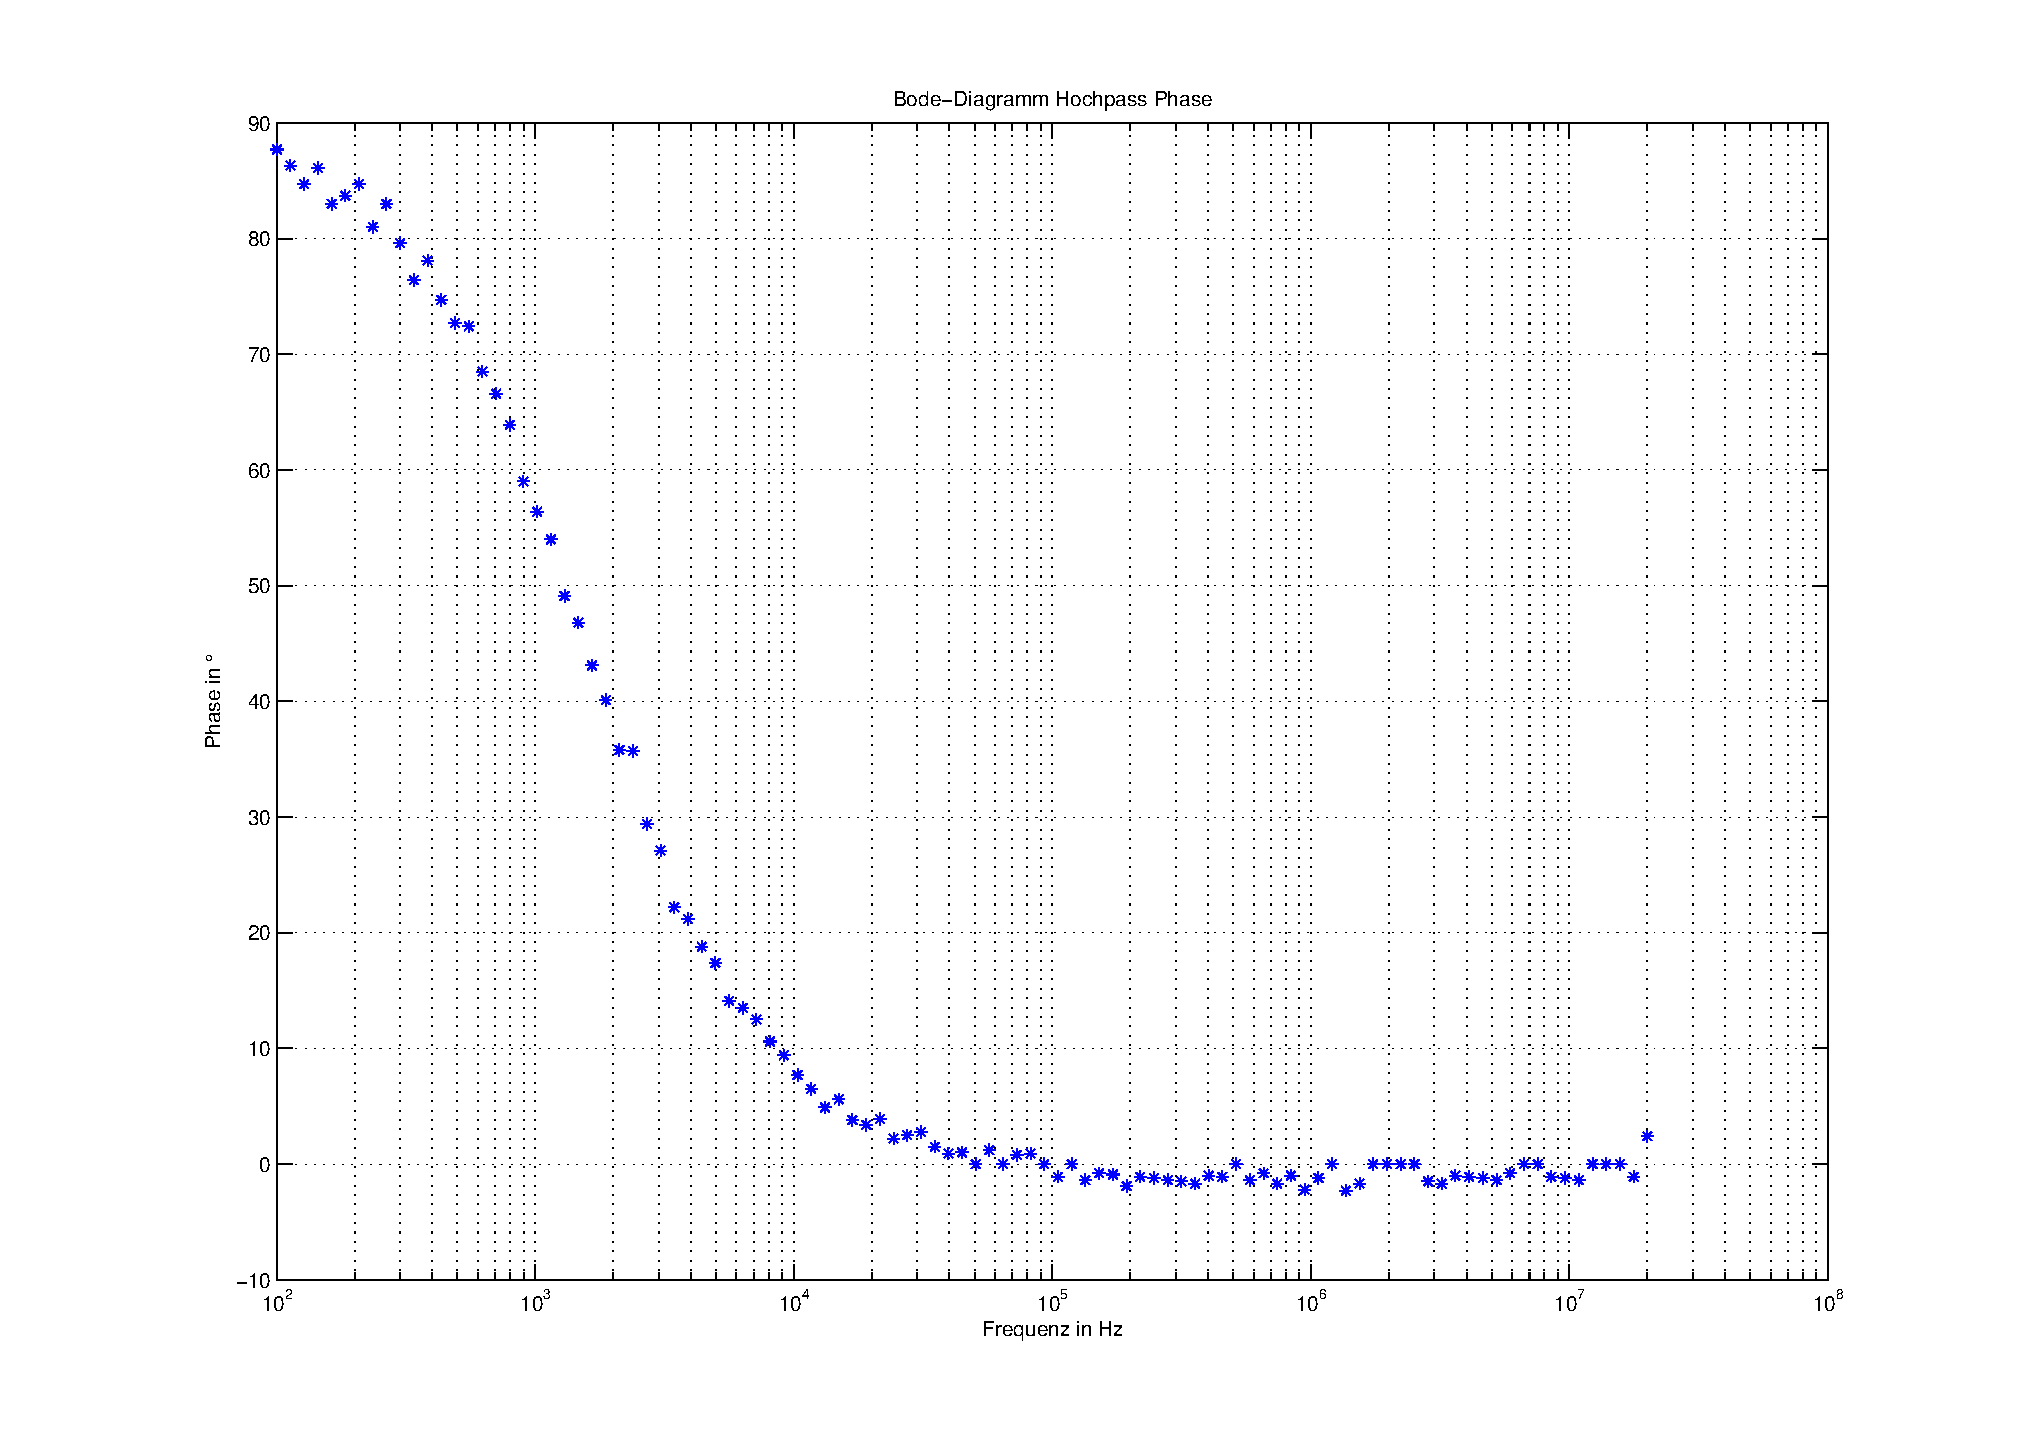
\includegraphics[scale=0.45]{./img/2b_bode_hoch_phase.eps}
     \end{center}
     \end{figure}
     \begin{itemize}
         \item Erwarteter Verlauf: 
     \end{itemize}
     \begin{equation*}
            \varphi = \arctan \left( \frac{1}{\omega C R} \right)
     \end{equation*}
\end{frame}
\begin{frame}
    \frametitle{Aufgabe 2}
    \framesubtitle{Hochpass 1. Ordnung}
    \begin{figure}[H]
    \begin{center}
            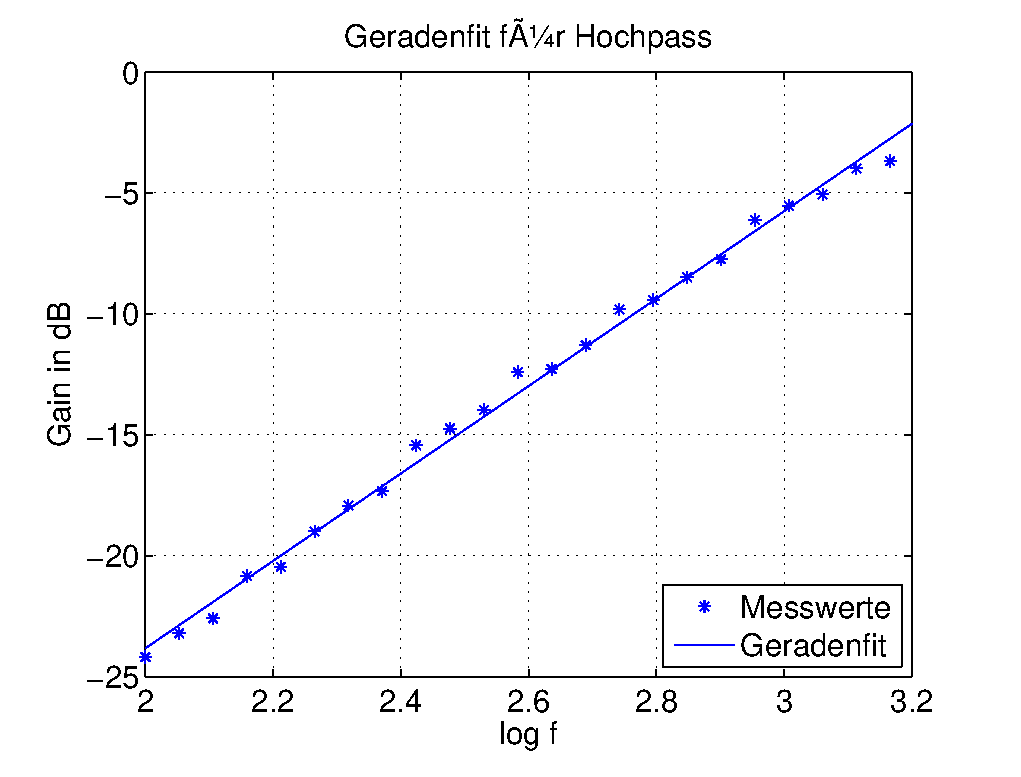
\includegraphics[scale=0.6]{./img/2b_Fit.eps}
    \end{center}
    \end{figure}
\end{frame}
\begin{frame}
    \frametitle{Aufgabe 2}
    \framesubtitle{Hochpass 1. Ordnung}
     \begin{itemize}
        \item Theoretische Grenzfrequenz: $f_{c_T} = \frac{1}{2 \pi C
        R}=1591.55Hz$ 
        \item Aus Bode Diagramm bei $dB=-3.398500$: $f_{c_T} \approx 1656 Hz$
        \item Fit Wert: $18.08 \frac{dB}{Dekade}= 5.42 \frac{dB}{Oktave}$
        \item Theoretischer Wert:
        $20\frac{dB}{\text{Dekade}}=6\frac{dB}{\text{Oktave}}$
     \end{itemize}
\end{frame}
\begin{frame}
\frametitle{Aufgabe 2}
\framesubtitle{AC-Modus des Oszilloskops}
\begin{figure}[H]
\begin{center}
        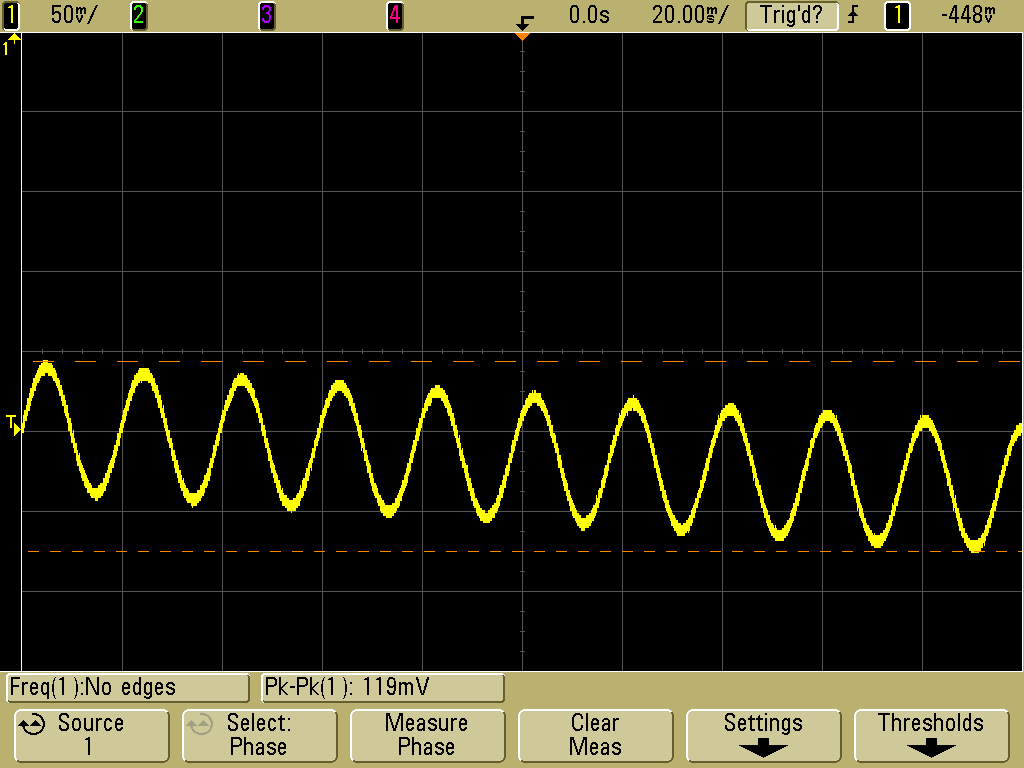
\includegraphics[scale=0.2]{./img/2c_Testsignal_1.png}
\end{center}
\end{figure}
\begin{itemize}
    \item Testsignal: Dreiecksspannung + Sinussignal
    \item Problem: Schwierigkeit bei automatischer Bestimmung der
    Amplitude - Sinus ist "schräg" und wandert
\end{itemize}
\end{frame}

\begin{frame}
\frametitle{Aufgabe 2}
\framesubtitle{AC-Modus des Oszilloskops}
\begin{itemize}
    \item Lösung 1: Vorschaltung eines Hochpassfilters
    \item Dreickspannung ist niedrigfrequentes Signal $\rightarrow$ wird
    herausgefiltert
\end{itemize}
\begin{figure}[H]
    \begin{center}
            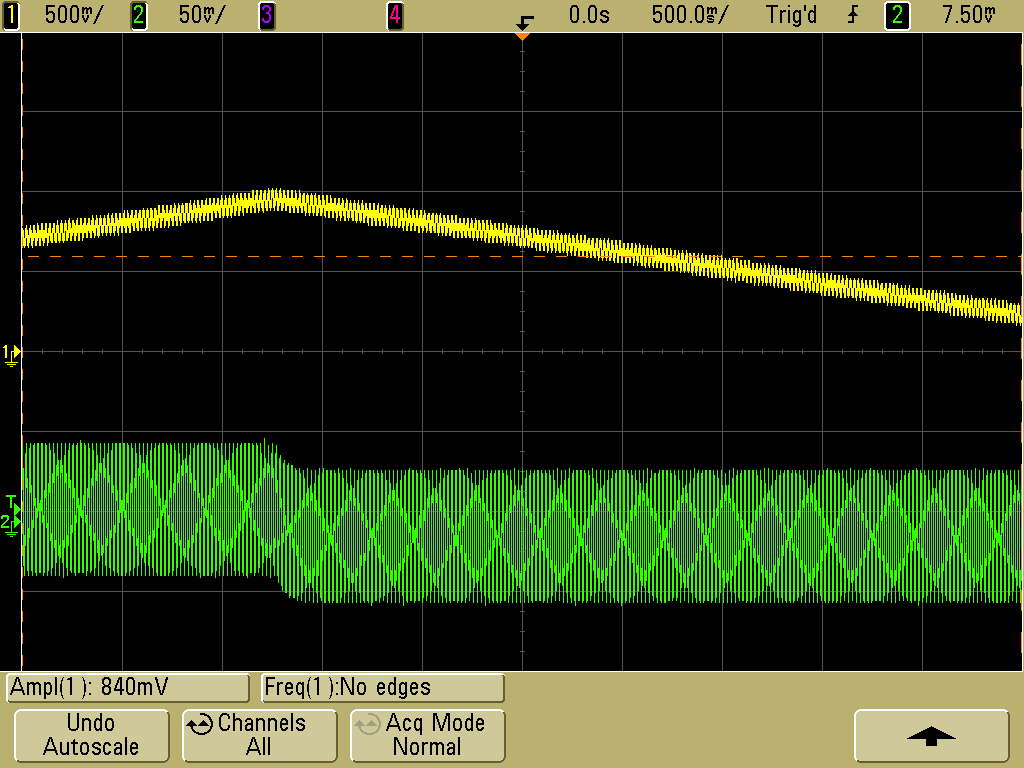
\includegraphics[scale=0.2]{./img/2c_Dreieck.png}
    \end{center}
\end{figure}
\end{frame}
\begin{frame}
    \frametitle{Aufgabe 2}
    \framesubtitle{AC-Modus des Oszilloskops}
     \begin{figure}[H]
     \begin{center}
             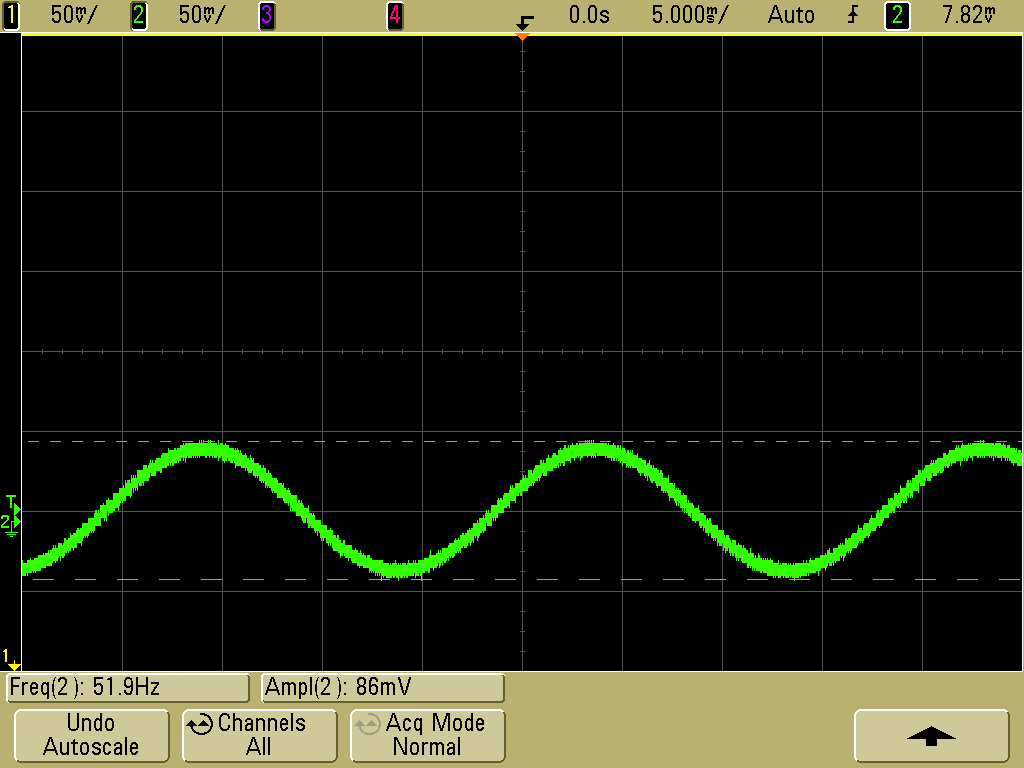
\includegraphics[scale=0.2]{./img/2c_Testsignal_mit_Hochpassfilter.png}
     \end{center}
     \end{figure}
     \begin{itemize}
        \item Frequenz: $f=51.9Hz$
        \item Amplitude: $\hat{U} = 86mV$
     \end{itemize}
\end{frame}
\begin{frame}
\frametitle{Aufgabe 2}
\framesubtitle{AC-Modus des Oszilloskops}
\begin{itemize}
    \item Lösung 2: Eingang auf AC-Modus
    \item eingebauter Hochpassfilter 
    \item Verwendung zum Filtern niedrigfrequenter Störungen
\end{itemize}
\begin{figure}[H]
\begin{center}
        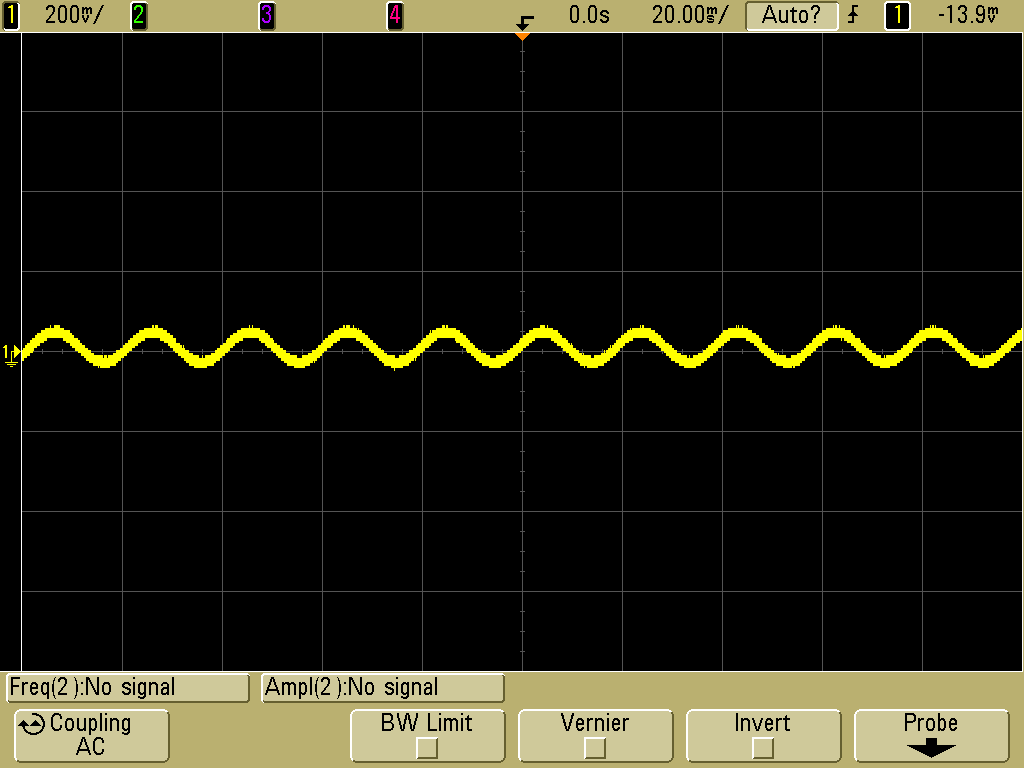
\includegraphics[scale=0.2]{./img/2c_Testsignal_AC.png}
\end{center}
\end{figure}
\end{frame}
